\documentclass[11pt]{article}
\usepackage{euscript}

\usepackage{amsmath}
\usepackage{amsthm}
\usepackage{amssymb}
\usepackage{epsfig}
\usepackage{xspace}
\usepackage{color}
\usepackage{url}

%%%%%%%%%%%%%%%%%%%%%%%%%%%%%%%%%
\setlength{\textheight}{9in}
\setlength{\topmargin}{-0.600in}
\setlength{\headheight}{0.2in}
\setlength{\headsep}{0.250in}
\setlength{\footskip}{0.5in}
\flushbottom
\setlength{\textwidth}{6.5in}
\setlength{\oddsidemargin}{0in}
\setlength{\evensidemargin}{0in}
\setlength{\columnsep}{2pc}
\setlength{\parindent}{1em}
%%%%%%%%%%%%%%%%%%%%%%%%%%%%%%%%%


\newcommand{\eps}{\varepsilon}

\renewcommand{\c}[1]{\ensuremath{\EuScript{#1}}}
\renewcommand{\b}[1]{\ensuremath{\mathbb{#1}}}
\newcommand{\s}[1]{\textsf{#1}}

\newcommand{\E}{\textbf{\textsf{E}}}
\renewcommand{\Pr}{\textbf{\textsf{Pr}}}

\title{Final Project Report: Importance-Sensitive Bloom Filters
\footnote{\s{CS 6955 Data Mining; \;\; Spring 2012 \hfill
Instructor: Jeff M. Phillips, University of Utah}
}
}
\author{Chad Brubaker \& Alex Clemmer}

\begin{document}
\maketitle





%%%%%%%%%%%%%%%%%%%%%%%%%%%%%%%%%%%%%%%%%%%%%%%%%%%%
%%%%%%%%%%%%%%%%%%%%%%%%%%%%%%%%%%%%%%%%%%%%%%%%%%%%
%%%%%%%%%%%%%%%%%%%%%%%%%%%%%%%%%%%%%%%%%%%%%%%%%%%%

\section*{Abstract}

A Bloom filter is a space-efficient representation of an arbitrary set that allows for probabilistic membership queries, providing an $\epsilon$-small one-sided probability of false positive.

One problem with the traditional Bloom filter is that this probability of error is always the same for all possible membership queries. However, the assumption that all elements \textit{should} have the same probability of error is inappropriate in many cases, particularly so in situations where the accuracy of the set membership query for certain elements is vastly more important than it is for others.

In this report we will demonstrate that it is possible to drive down the error selectively for ``important" elements in the set by adjusting the number of hash functions used to test set membership. We will also begin to pin down the analysis of the guarantees that can be provided by the techniques we outline.

\section{Motivation}

On a purely practical basis, it is not at all uncommon for data to exhibit a Zipf-like trend in the real world, which historically has meant that actionable knowledge that provides realistic tools for dealing with sparse feature distributions tend to be very welcome, especially in domains where experiments tend to be very memory-intensive (\textit{e.g.}, NLP and ML).

Our motivation specifically was to make it possible to do machine learning algorithms using massive amounts of natural language data, but using only commodity computers. Recent algorithmic advances have undoubtedly made this much easier, but our progress was nevertheless still impeded by the fact that the long tail of features washed out accuracy for the very important features, and this was the inception of the techniques presented here.

\section{Problem Statement}

We adopt the traditional notation for Bloom filters. That is, the classical Bloom filter represents an arbitrary set of $n$ elements $S = \{ s_1, \ldots, s_n \}$, and consists of two basic components: (1) an $m$-bit array $A$, where all bits are initially set to 0, and (2) a set of $k$ hash functions $H = \{ h_1, \ldots, h_k \}$, where each hash function $h_i : \mathbb{R^d} \rightarrow \mathbb{N}$ maps integers into the range $[0,m)$.

\subsection{Background on the Bloom Filter}

The Bloom filter represents a particular $s_i \in S$ first by feeding it into each of the $k$ hash functions. Each particular hash function $h_j \in H$ will produce an integer value, for a total of $k$ integer values. For each of these $k$ integer values, we set $A[h_j(s_i)] = 1$, \textit{i.e.}, we treat each of the $k$ values as an index into $A$, and at each of these $k$ points in $A$, we set the value to 1 (note that we set it to 1 even if it has already been set to 1 beforehand!).

This leaves us the problem of checking set membership. Let's call our query point $q_i$. Similar to the above, we begin be feeding $q_i$ into each of the $k$ hash functions to get $k$ integer values. However, unlike above, we don't set any values in $A$---instead, we check to see that each of the $k$ value in $A$ is set to 1. If all $k$ of the values are set to 1, we conclude that $q_i$ is in the set $S$; otherwise, we conclude that it is not.

\subsection{Error Rates in Bloom Filters}

Bloom filters have one-sided error, \textit{i.e.}, they are only capable of producing false positives. Thus, our job in this paper will be to \textit{reduce the probability of false positives on a selective basis}, and as such it will be useful to characterize the false positive rate of the generic Bloom filter as a starting point.

Classically, the probability of any particular bit being set to one in an $m$-bit Bloom filter representing an $n$-element set using $k$ hash functions is denoted by

\begin{equation}
\mathcal{E} = 1 - \left(1 - \cfrac{1}{m} \right)^{nk}
\end{equation}

Another way to think of this is as the probability that all the bits except one particular bit are \textit{not} flipped, over $k$ hash functions and $n$ different items. Another classic result gives us the false positive rate:

\begin{equation}
\text{error}(k) = \mathcal{E}^k = \left( 1 - \left( 1 - \cfrac{1}{m} \right)^{nk} \right)^k
\end{equation}

\subsection{Establishing a Notion of ``Importance"}

In addition to the set $S$ let us adopt $Q = \{ q_1, \ldots, q_p \}$ to indicate our set of $p$ query points. Generically, we'd like to attach to each of these points a measure of \textit{importance}, which we will eventually optimize to find the allocation of hash functions that most greatly reduces the probability of false positives.

Formally, this can be represented as a function $I : \mathbb{R}^d \rightarrow \mathbb{R}$, which takes a query point and maps them to real-valued importance scores.

At the outset, this formulation should be worrying---$I$ is assigning real-valued importance scores to each of the query points in the set $Q$, but what we really need is a natural number that we can optimize to tell us how many hash functions to allocate to a particular point. After all, if you have ranked your importance for some query point as 2.73, you are sort of stuck because it doesn't make any sense to allocate 2.73 hash functions. This looks dangerously like an (Integer Programming) IP problem.

Unfortunately, it is necessary to formulate $I$ in this way for the sake of generality. Consider, for example, the very likely scenario that $I$ is a function that operates on a probability distribution, such as the probability that a particular query point is queried. The simple fact of the matter is that there are many reasonable choices for $I$ that are not integer-valued, and in order to not lose generality, we must ultimately confront this issue.

\subsection{Possible Programs for Optimizing Hash Allocation}

The problem that remains is to formulate a systematic way for determining how many hash functions should be allocated to each member of the set.

The first and most obvious way to perform this optimization is to simply round the real-valued importance $I(q_i)$ (for each particular $q_i \in Q$) to the nearest integer. Historically, this sort of optimization program tends to do poorly both in theory and in practice compared to the empirical optimum, and this tends to be enough motivation to seek a different formulation of the problem.

Another option is to simply solve the IP. This sort of practice tends to be acceptable in ML circles as long as the program runs ``fast enough"; one reason this might be a realistic choice for our purposes (\textit{i.e.}, for use in ML) is the fact that the number of hash functions used in Bloom Filters in ML (\textit{e.g.}, for counting features) tends to be small, which means it is likely that the IP will complete in a reasonable amount of time.

This will make some theoretical CS people upset; for our purposes, however, it will do fine, and our remaining problem is how to present this as an IP minimization.

\subsection{Formulating the IP Minimization}

Our first trick is to partition our query set $Q = \{ q_p \}$ into two groups: (1) let $F \subseteq Q$ represent the queries that are reported as false positives, \textit{i.e.}, the queries points that are \textit{not} in $S$, but which are reported as in $S$ anyway; and (2) let $P \subseteq Q$ represent the group of queries that are actually in $S$.

First, observe that normalizing the importance score over both of these subsets gives us a probability distribution on that subset, \textit{i.e.},

\begin{eqnarray}
\sum_i^n \cfrac{I(q_i)}{n} = 1, & \forall q_i \in P,
\end{eqnarray}

where $n$ (in this particular case) represents the number in the subset $P$. Obviously the Kolmogorov axioms hold here, and trivially this all applies for $F$. Now, if we are given a budget of hash operations to use $\mathcal{B}$, then from here we have an IP minimization problem.

\begin{eqnarray}
\text{minimize} & \sum_i^p I(f_i) \cdot \text{ error}(k_i), & \forall f_i \in F \\
\text{subject to} & \sum_i^p I(p_i) \cdot k_i = \mathcal{B}, & \forall p_i \in P
\end{eqnarray}

Transforming this to a Lagrangian function (with a single Lagrange multiplier) is trivial:

\begin{eqnarray}
L(\lambda) = \sum_i^n I(f_i) \cdot \text{ error}(k_i) - \lambda(\sum_i^p I(p_i) \cdot k_i - \mathcal{B}) & \forall f_i, p_i \in F \times P
\end{eqnarray}

Neither of us have any experience with non-convex optimization, nor are we especially capable theoreticians, so we will save ourselves embarrassment and just mention that existing IP libraries (\textit{e.g.}, MIPLIB, POLIP, \textit{etc.}) made formulating this as a computer program relatively easy.

\section{Application and Evaluation}

To see why the above program makes sense, it may be helpful to consider the case where we view the most ``important" items as being the items that are simply queried the most. In this case, the importance function $I$ would give us the probability that a particular query point $q_i$ is queried, which means that this formulation essentially optimizes probability of false positives for the popular queries.

Of course the fact that we don't inherently specify $I$ means that our optimization program is generic to whatever the user wants to optimize, but this turns out to be a good illustrative example for the way the problem works, because it is also exactly the model we use experimentally in this report, over both our datasets.



\subsection{SemEval 2012 Results}

\textit{*** Note: Due to hard drive failure part of the way through the project, the SemEval data was lost; this is one reason why there are two datasets.}


The first of our two datasets is the \textit{SemEval 2012 spatial role labeling shared task dataset}. Spatial role labeling tends to refer to the task of analyzing free text to determine relationships between objects, \textit{e.g.}, a cup might be on top of a table.

This sort of analysis tends to be extremely tricky, and our experiments pertain exclusively to representing features after extraction. For simplicty, we have chosen to use the existing feature extraction gold standard in order to allow us to concentrate on representing the features efficiently. In particular, we will \textit{not} concentrate on the task of extracting the features themselves (a significant problem), or on actually performing this labeling task itself. We are only on dealing with the representation of the features associated with this task using the methods previously described.

Formalities aside, fitting a line to the feature count histogram reveals the following pattern:

\begin{center}
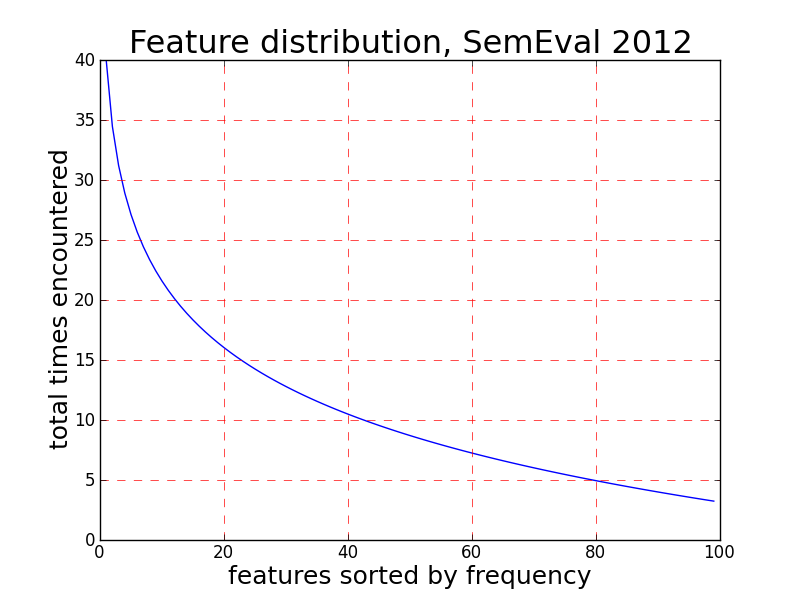
\includegraphics[scale=0.25]{dist1.png}
\end{center}


The classical way to compare the results of the Bloom filter's performance is to vary the ratio of the size of the filter $m$ to $n$, the number of elements in $S$. A plot describing what happens as the ratio is changed follows:

\begin{center}
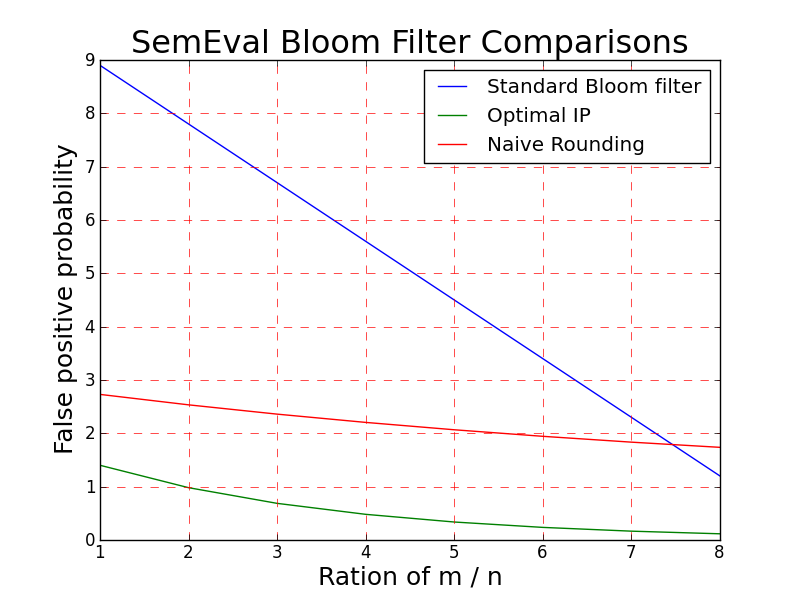
\includegraphics[scale=0.25]{resultsse.png}
\end{center}

The ``standard" Bloom filter implementation pretty clearly declines at a steady but unsatisfying rate---only when $m$ is nine times the size of $n$ does its probability of false positive drop to the point where it becomes a feasible competitor to either of the rounding methods. It does, however, notably out-perform the naive rounding filter.

On the other hand, the naive rounding actually seems to give a good approximation of the IP optimum. This may carry a distinct advantage because, although we did not plot it, it also took \textit{much less} time. It is unlikely that you'll want to construct a filter large enough that the standard type becomes better, so this may be a winning method overall.

In terms of raw performance, it is pretty clear that the optimum is indeed the optimum. This happens to be by a margin of a few percentage points, so it is probably suited only to applications where either space or accuracy are \textit{much} more important than running time.





\subsection{Twitter MITRE Results}

The second dataset is a glob of proprietary \textit{Twitter data} that Alex obtained via an ongoing extra-institutional RA position he holds at Johns Hopkins University.

The data is used in ongoing research that seeks to use purely-streaming algorithms to identify gender, and the feature extraction process is already in place. Again we depend on this existing pipeline to provide us features opaquely; rather than reciting how these features are selected, we will concentrate specifically on how to effectively represent features that aid in the task.

In this case, fitting a line to the feature count histogram reveals a much more biased distribution than the SemEval data:

\begin{center}
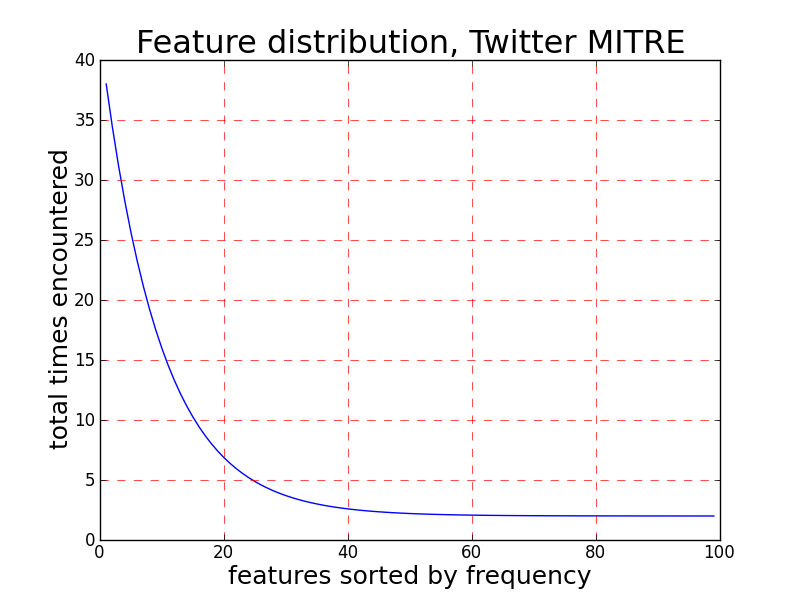
\includegraphics[scale=0.25]{dist2.png}
\end{center}

Again we use the ratio of $m$ to $n$ to compare the performance of our filters.

\begin{center}
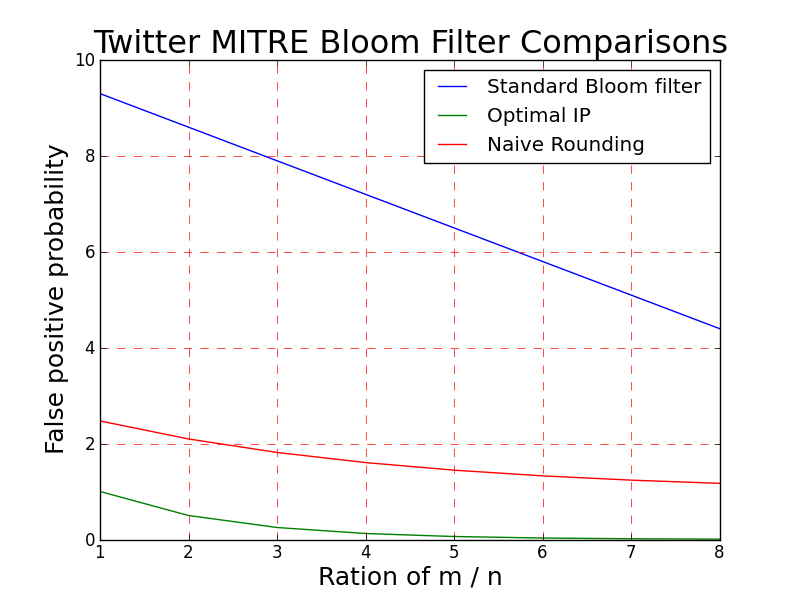
\includegraphics[scale=0.25]{resultst.png}
\end{center}

This result is actually harder on everyone. It might be unintuitive until you consider that, classically, we know that $\text{error}(k)$ is minimized when the probability of any particular bit being flipped $\mathcal{E} = \frac{1}{2}$, in which case it would make sense that skewed feature distributions would cause the results generally to suffer.

The obvious changes are in the naive rounding and ``standard" filter schemes, which both suffer overall, even as the ratio of $m$ and $n$ becomes greater. In contrast, the clear winnder is the IP optimum, which actually does even better than on the last dataset---it actually peters out to very small values much faster than either of the other two.

Unfortunately, it is also true that the IP optimum to longer to run---at least 15 minutes on our wimpy machines. The Twitter dataset is probably 10 times larger than the SemEval dataset, but it is has lower dimensionality. It's not a part of our analysis, but it is worth noting for people who are thinking of using this scheme.


\section{Conclusions}

The strong conclusions to take away here are that spending the time to take the IP optimum does cost you in time, but what you tend to gain is a stable, vastly more space-efficient representation of you set $S$. The naive Bloom filter often was an order of magnitude worse, for the lower ratios of $m / n$, for example.

The downsides are that naive seems to give adequate performance in many cases---it usually gets around 1-2\%, which is intuitively not bad. Unfortunately, intuition is not really the best tool for judging whether this is a good or bad mark, and this becomes especially obvious if you think about working on larger datasets. As a simple example, if your hard drive failed had a bit-error rate of 1\%, it is doubtful that you would be able to run it for more than a couple hours before some critical part of the operating system failed. In fact, the typical error rate for hard drives is somewhere in the ballpark of $10^{-13}$\%, which should illustrate the problem with being consistently exposed to the probability of error over time.

The IP optimum may take time, but if you're dealing in an area like the last example and are worried about performance issues, it is presents the possibility of driving error to very small percentages, which is a distinct advantage over the other two systems (in which this is not really possible in a practical setting).

One promising area of research would be to look at different ways of conducting the IP. Our solution is naive, but there are probably other ways of solving the IP that are faster, and probably, that allocate functions better. Our approach sort of assumes a bounded error approximation, and the details of what we assumped can and should be challenged.

This, of course, is to say nothing of the basic problems we left on the floor. The explicit optimum for the IP remains to be shown, for example. Another interesting question is how fast this is actually guaranteed to run in---we know it's exponential, but the question is according to what factors.

Most exciting by far, though, is that this technology has born out well enough that we realistically are one step closer to truly-streaming algorithms on massive, sparse datasets, such as those that are extremely commonly found in NLP. The real promise of research like this is that it gradually is pushing towards to solutions that we are really just now staring to be forced to grapple with. It's hard to imagine the problems of massive data will simply vanish tomorrow, and any progress at in any area that can help us address these problems on a practical basis (and especially on commodity machines) are most welcome.


\section{Work Divisions}

As a matter of technicality, we completed most of the work sitting right next to each other. The code was almost all written in person, in Python. Work that was not done right next to each other included reading, and assembling of data. Alex was wholly responsible for collection of both corpora, for identifying the problem, and for pointing out useful papers. But that's his job as a researcher anyway, and the gruntwork was completed by both partners simultaneously.











\end{document}
